\documentclass[t]{beamer}
\usepackage{CJKutf8}
\usepackage{amsfonts}
    \usepackage{amsmath}
    \usepackage{amssymb}
    \usepackage{amsthm}
    \usepackage{enumerate}
    \usepackage{graphicx}
    \usepackage{layout}
    \usepackage{mathrsfs}
    \usepackage{fancyhdr}
    \usepackage{subfigure}
    \usepackage{tcolorbox}
    \usepackage{tikz-cd}
    \usepackage{color}
    \usepackage{pifont}
    \usepackage{verbatim}
    \usepackage{mathtools}
    \usepackage{float}
    \usepackage{bm}
    \usetheme{AnnArbor}
% \usetheme{Antibes}
\usecolortheme{beaver}

% 添加网址的命令
\usepackage{hyperref}
% 这是一个带链接文本的示例:\href{https://www.example.com}{点击这里访问网站}
% 普通的示例:\url{https://www.example.com}
% 表格
\usepackage{booktabs}
\usepackage{multirow}

% \setbeamertemplate{navigation symbols}{}

\usepackage{textpos}

\newcommand{\dif}{\mathrm{d}}
\newtheorem{thm}{{定理}}

% some common command
\newcommand{\mm}[1]{$ #1$\newline}
% \newcommand{\tuichu}{\Rightarrow}
% \newcommand{\li}[1]{\newline#1}



\newcommand{\analysis}[2]{\forall \mathcal{E}{#1},\exists \delta {#2},s.t.}
\newcommand{\denyanalysis}[2]{\exists \mathcal{E}{#1},\forall \delta {#2},s.t.}
\newcommand{\yield}{\Rightarrow }
\newcommand{\jj}{\newline}
\newcommand{\ff}[1]{$ #1$}   % math environment + newline
\newcommand{\fgn}[1]{\begin{equation}#1\end{equation}  }
\newcommand{\fg}[1]{$$ #1$$}   % math environment + newline 
\newcommand{\pf}{$proof.$\newline}
\newcommand{\ee}{\newline\ff{\Box}\newline}
\newcommand{\fenshi}[2]{\ff{\frac{#1}{#2}}}
\newcommand{\shenlue}{\vdots\jj}
\newcommand{\abs}[1]{{\left \lvert #1 \right\rvert}}
\newcommand{\loge}[1]{In ({#1})}
\newcommand{\logical}[2]{log_{#2}^{#1}}
\newcommand{\summary}[3]{$\sum_{{#1}={#2}}^{#3}  $}
\newcommand{\denjia}[2]{{#1}\Leftrightarrow {#2}}
\newcommand{\jihe}[3]{ {#1}  = \{ {#2} \mid {#3} \} }
\newcommand{\ve}[2]{\left\langle {#1},{#2}\right \rangle}
\newcommand{\dakuohao}[2]{\begin{array}{rcl}{#1}\end{array} \} \Rightarrow{#2}}
\newcommand{\sxb}[3]{#1^{#2}_{#3}}
\newcommand{\sss}[2]{#1^{#2}}
\newcommand{\xxx}[2]{#1_{#2}}
\newcommand{\bri}[1]{\uppercase\expandafter{\romannumeral#1}}
\newcommand{\ri}[1]{\romannumeral#1} 
\newcommand{\polynomial}[8]{#1_{#2}#6^{#7}+#1_{#3}#6^{#8}+...+#1_{#4}#6+#1_{#5} }
\newcommand{\newd}[4]{f[{#1}_{#2},{#4},{#1}_{#3}]}
\newcommand{\lb}[2]{\begin{align*}\begin{split}{#1}\{ {#2}\end{split}\end{align*}}
\newcommand{\tab}[1]{\begin{array}{ll} {#1}\end{array}}


% 向量乘积
\newcommand{\avg}[1]{\left\langle #1 \right\rangle}
% 偏微分方程
\newcommand{\difFrac}[2]{\frac{\dif #1}{\dif #2}}
\newcommand{\pdfrac}[2]{\frac{\partial{#1}}{\partial{#2}}}
% 不同章节
\newcommand{\one}[1]{\section{#1}}
\newcommand{\two}[1]{\subsection{#1}}
\newcommand{\three}[1]{\subsubsection{#1}}
\newcommand{\aone}[1]{\section*{#1}}
\newcommand{\atwo}[1]{\subsection*{#1}}
\newcommand{\athree}[1]{\subsubsection*{#1}}
% 大括号,左右都有
\newcommand{\lbra}[1]{\left\{  {\begin{matrix} #1 \end{matrix}}\right. } 
% 样式 括号前缀 + 括号 
\newcommand{\lbras}[2]{{#1}\left\{ {  {\begin{matrix} #2 \end{matrix}}}\right. } 
\newcommand{\rbra}[1]{ \left.  {\begin{matrix} #1 \end{matrix}} \right\}  } 
% 模长
\newcommand{\distance}[1]{\parallel #1\parallel }
% 等价
\newcommand{\equ}{\Longleftrightarrow }
% 共轭
\newcommand{\cja}[1]{\overline{#1}}
% 两个矩阵,上面是 方框[] 下面是线条| 中间是 无
\newcommand{\mtx}[1]{\begin{matrix}#1\end{matrix} }
\newcommand{\bmtx}[1]{\begin{bmatrix}#1\end{bmatrix} }
\newcommand{\vmtx}[1]{\begin{vmatrix}#1\end{vmatrix} }
% \newcommand{\table}[1]{\begin{array}[lr]{ccc} #1 \end{array}}

%输入普通字符
\newcommand{\ww}[1]{\text{#1}}

% 所有内容 直接头文件搞定
\newcommand{\everything}[1]{\begin{document}\begin{CJK*}{UTF8}{gkai}#1\end{CJK*}\end{document}}


% 存放代码(失败了)
\newcommand{\cccode}[1]{\begin{lstlisting}#1\end{lstlisting}}

% 改变特定行序列
\newcommand{\ttt}{\subsection{}}

% 嵌套序号
\newcommand{\eee}[1]{\begin{enumerate}#1\end{enumerate}}


% 模板里面的一些宏
\newcommand{\pdfFrac}[2]{\frac{\partial #1}{\partial #2}}
\newcommand{\OFL}{\mathrm{OFL}}
\newcommand{\UFL}{\mathrm{UFL}}
\newcommand{\fl}{\mathrm{fl}}
\newcommand{\op}{\odot}
\newcommand{\Eabs}{E_{\mathrm{abs}}}
\newcommand{\Erel}{E_{\mathrm{rel}}}
% 变化颜色
\newcommand{\red}{\textcolor{red}}
\newcommand{\blue}{\textcolor{blue}}



% 流程图需要用到的宏包
\usepackage{palatino}
\usepackage{tikz}
\usetikzlibrary{shapes.geometric, arrows}
\tikzstyle{startstop} = [rectangle, rounded corners, minimum width = 2cm, minimum height=1cm,text centered, draw = black, fill = red!40]
\tikzstyle{io} = [trapezium, trapezium left angle=70, trapezium right angle=110, minimum width=2cm, minimum height=1cm, text centered, draw=black, fill = blue!40]
\tikzstyle{process} = [rectangle, minimum width=3cm, minimum height=1cm, text centered, draw=black, fill = yellow!50]
\tikzstyle{decision} = [diamond, aspect = 3, text centered, draw=black, fill = green!30]
% 箭头形式
\tikzstyle{arrow} = [->,>=stealth]
% 4个非常重要 的新命令
\newcommand{\start}[2]{    \node (start) [startstop]{#1};\node (in1) [io, below of = start]{#2};\lin{start}{in1}{}}
\newcommand{\stopp}[3]{\node (out1) [io, below of= #1]{#2};\node (stop) [startstop, below of=out1]{#3};\lin{out1}{stop}{} }
\newcommand{\pro}[6]{    \node (#3) [process, #2 of=#1,xshift=#4 cm]{#5};}
\newpage
\newcommand{\lin}[3]{\draw [arrow] (#1) --node [above] {#3} (#2);}


\begin{document}
\begin{CJK*}{UTF8}{gkai}
% 一般第一页显示PPT标题以及作者信息

% \BackgroundPic{./Screenshot from 2022-04-20 16-31-08.png}

% 增加学校 前面
\addtobeamertemplate{title page}{}{
	\begin{tikzpicture}[remember picture,overlay]
		% \node[yshift=85pt,xshift=50pt]{\includegraphics[height=2cm]{Screenshot from 2022-04-20 16-51-21.png}};
\end{tikzpicture}
}


	\title{大型语言模型(LLM)}
	\subtitle {} %不需要
	\author{
		陈钶杰\, \\
		专业:计算数学\,
	} % 显示作者
	% \institute {学院:数学科学学院} % 设置学院机构	
	\date{\today}  % 显示日期
\titlepage

% 设置目录
\begin{frame}{目录}
\frametitle{目录}	
\tableofcontents  % 显示目录
\end{frame} 



\section{NLP模型综述}  

\subsection{大型语言模型(LLM)的技术精要}

\begin{frame}
	\frametitle{LLM模型}
    \begin{itemize}
		\item 
		\textcolor{red}{解决一下几个问题}
		\begin{itemize}
		\item ChatGPT是否带来了NLP乃至AI领域的研究范式转换?
		% \item 如果是,那会带来怎样的影响?
		\item LLM从海量数据中学到了什么知识?
		\item LLM又是如何存取这些知识的?
		\item 随着LLM规模逐步增大,会带来什么影响?
		\item 什么是In Context Learning?
		% \item 为什么它是一项很神秘的技术?
		% \item 它和Instruct又是什么关系?
		% \item LLM具备推理能力吗?
		% \item 思维链CoT又是怎么做的?等等,相信看完,能让您对这些问题有一个答案。
		\end{itemize}
	\end{itemize}
\end{frame}

\begin{frame}
	\frametitle{ChatGPT是否带来了NLP乃至AI领域的研究范式转换?}
	% \includegraphics*[scale=0.2]{png/all_prompt.png}
	\textcolor{red}{目前规模最大的LLM模型,几乎都是类似GPT 3.0这种“自回归语言模型+Prompting”模式的.}	\\
	原因如下:
		\eee{
			\item 可以把分类问题转换成让LLM模型生成对应类别的字符串,这样理解和生成任务在表现形式就实现了完全的统一。同一个LLM生成模型,可以解决几乎所有NLP问题。而如果仍然采取Bert模式,则这个LLM模型无法很好处理生成任务。
			\item 如果想要以零示例提示语(zero shot prompting)方式做好任务,则必须要采取GPT模式。有研究证明:如果是以fine-tuning方式解决下游任务,Bert模式的效果优于GPT模式;若是以zero shot/few shot prompting这种模式解决下游任务,则GPT模式效果要优于Bert模式。这说明了,生成模型更容易做好zero shot/few shot prompting方式的任务,而Bert模式以这种方式做任务,是天然有劣势的。
		}
\end{frame}

\begin{frame}
	\frametitle{ChatGPT是否带来了NLP乃至AI领域的研究范式转换?}	
	\textcolor{red}{本来我们希望LLM能够用人类常用的命令方式来执行某个任务,但是目前技术还做不到,所以退而求其次,用Instruct技术来表达人类的任务需求。}
	\eee{
			\item ChatGPT的出现,改变了这个现状,用Instruct取代了Prompting,由此带来新的技术范式转换,并产生若干后续影响.
			\item 基本实现了理想LLM的接口层,让LLM适配人的习惯命令表达方式,而不是反过来让人去适配LLM,绞尽脑汁地想出一个能Work的命令(这就是instruct技术出来之前,prompt技术在做的事情),而这增加了LLM的易用性和用户体验。相对之前的few shot prompting,它是一种更符合人类表达习惯的人和LLM进行交互的人机接口技术。
		}
\end{frame}


\begin{frame}
	\frametitle{LLM相关的知识}
	\textcolor{red}{LLM学到了什么知识}	
	\eee{
		\item 语言类知识:词法、词性、句法、语义等有助于人类或机器理解自然语言的知识。
		% 人类或机器理解的知识
		\item 世界知识: 在这个世界上发生的一些真实事件,以及一些常识性知识。
		% 常识性知识
	}
	\textcolor{red}{LLM如何存取知识?}	
	\eee{
		\item 知识存储是在Transformer模型的参数里面的,1/3数据在多头注意力,2/3数据在FFN结构中.所以知识主体是存储在FFN结构里面的.\\
		% 举个例子:当tranformer中key向量用于检测输入是"中国的首都是[mask]",value向量则对应的单词embedding基本就是北京了.
	}
	\textcolor{red}{LLM的规模}	
	\eee{
		% \item 我们可以选择放大训练数据,并同比例地减少LLM模型参数,以达到在不降低模型效果的前提下,极大缩小模型规模的目的。缩小模型规模有很多好处,比如在应用的时候,推理速度会快很多等,无疑这是一个很有前途的LLM发展路线。
		\item “涌现能力”:指的是当模型参数规模未能达到某个阀值时,模型基本不具备解决此类任务的任何能力,体现为其性能和随机选择答案效果相当,但是当模型规模跨过阀值,LLM模型对此类任务的效果就出现突然的性能增长
	}
\end{frame}

\begin{frame}
	\frametitle{人机接口:从in context learning到instruct理解}
	\textcolor{red}{仔细区分这些不同的人机接口}	
		\eee{
			\item In Context Learning只是拿出例子让LLM看了一眼,并没有根据例子,用反向传播去修正LLM模型参数的动作,就要求它去预测新例子。	
			\item 早期大家做zero shot prompting,实际上就是不知道怎么表达一个任务才好,于是就换不同的单词或者句子,反复在尝试好的任务表达方式,这种做法目前已经被证明是在拟合训练数据的分布.
			\item Instruct的做法则是给定命令表述语句,试图让LLM理解它。所以尽管表面都是任务的表述,和zero shot prompting思路是不同的。
		}
\end{frame}


% \subsection{大模型微调需要多少数据}

% \begin{frame}
% 	\textcolor{red}{浅层对齐假说}	
%     \begin{itemize}
% 		\item 一个模型的知识和能力几乎完全是在预训练中学习的,而对齐则是教它在与用户交互时应该使用哪种子分布的格式。
% 	\end{itemize}
% 	% \textcolor{red}{微调数据规模并不需要那么多,就可以达到一个不错的效果}	
% 	% \begin{itemize}
% 	% 	\item 在1000个精心策划的例子上对一个强大的预训练语言模型进行微调,可以在广泛的提示中产生显著的,有竞争力的结果.
% 	% \end{itemize}
% 	\textcolor{red}{结论}	
% 	\begin{itemize}
% 		\item 多样性,高质量这两个数据上的问题一直被认定是决定模型性能的天花板。
% 		\item 在目前的绝大多数微调模型,都是靠着大力出奇迹来实现一个较好的性能,这也是过去几个月大家都在卷数据量的一个真实写照。
% 		\item 但是否想过,openai这种什么技能都能做到的模型,在多样性上应该做了大量的工作,并且在数据量上应该没有太大的追求。
% 		\item 所以,最近的风向变成,是否可以利用少量的数据就能取得差不多的效果,这样的话,努力的方向就可以变成多样性数据的挖掘上,这可能是openai走通但我们没想明白的地方。
% 	\end{itemize}
% \end{frame}

% \begin{frame}
% 	\frametitle{决定大模型能力的关键因素}
% 	\textcolor{red}{模型参数还是训练文本的大小?}
%     \begin{itemize}
% 		\item PalM2选择后者为主要路径,文本数量是训练其前身模型的5倍.
% 		\item 微软的新模型Bard和chat GPT类似的存在,也是非常的强大.
% 	\end{itemize}
% \end{frame}


\subsection{压缩即智能?}

\begin{frame}
	\frametitle{如果大语言模型具备越强的数据压缩能力,是否意味着它具备越强的AGI智能呢?}	
	\textcolor{red}{数据压缩:压缩即智能}
    \begin{itemize}
		\item GPT模型训练的过程就是在进行数据压缩,将输入的语句等以参数的形式保存.比如Large Language Model Meta AI(LLAMA)模型的数据压缩率在14倍左右.
		\eee{
			\item "最小描述长度原理"可以用来解释这个观点.
			\item 比如我输入一个长度为1万的质数序列"2,3,5,11,...",那么对于这个输入的最佳解释即要尽可能短而准确的描述这个序列,比如输出"从2开始的一万个连续质数".\\
			% 我的理解是"从2开始的一万个连续质数"即是LLM模型把输入转化成的参数.
		}
		\item LLM的这种数据压缩能力是无损的.\\
		\eee{
			\item 此模型能根据上文Context,给出的后续Next Token肯定会有错误,这些被预测错误的Token,其实就代表了LLM压缩数据的信息损失,这种损失是靠算术编码额外对信息进行编码来进行补偿,才达成数据的“无损压缩”效果.即有如下的公式:\\
			\item 数据无损压缩=LLM模型的有损数据压缩能力+算数编码的补偿能力
		}
	\end{itemize}
	% 	\textcolor{red}{最小描述长度原理}
	% 	\begin{itemize}
	% 		\item 假设有很多模型可以对手上的数据进行描述,那么最佳解释就是尽可能短且精确的描述.
	% \end{itemize}
	% \textcolor{red}{GPT模型学习知识的顺序?}
	% \begin{itemize}
	% 	\item 高频知识点
	% 	\item 通用知识点
	% 	\item 具体而非抽象的知识点
	% \end{itemize}
\end{frame}
\subsection*{模型差异}

\begin{frame}
	% \frametitle{大LLM模型和小LLM模型的差异}	
	\textcolor{red}{大LLM模型和小LLM模型的差异}	
	% {小LLM模型建立了一个粗粒度的,模糊的世界图像,而随着模型规模越来越大,大LLM模型建立起能表征更多细节信息的清晰度越来越高的世界图像.}	
    \begin{itemize}
		\item 小LLM模型建立了一个粗粒度的,模糊的世界图像,而随着模型规模越来越大,大LLM模型建立起能表征更多细节信息的清晰度越来
		越高的世界图像.
	\end{itemize}
	\textcolor{red}{回路竞争视角下的tuning}
	\begin{itemize}
		\item "回路竞争"猜想:如果从低向上激发过程中,我们希望的正确回路被激发,可以认为回路竞争胜利,则模型输出正确答案,而如果错误任务回路被激发,可以认为回路竞争失败,则模型输出错误答案。
		% \item 比如我给了一个机器翻译的任务,输入经过逐个层后输出,这个输入在最开始的几层,可能会和其他任务(比如文本分类)的回路重叠,通过不断前进,重叠会不断变少,越到上层这个重叠会越少,最终得到机器翻译的输出.
		\item 可能通过Fine-tuning操作,在模型内部建立起了Shortcut捷径,导致输入信息后,信息传输直接走了捷径,而绕过了很多本该要走的通路。
		% \eee{
			% \item Fine-tuning操作通过大量领域数据,强化了大语言模型解决这个任务的响应回路。这对于模型底层知识点影响估计不大,因为底层更多的是通用性比较强的特征,这个任务也需要,它修正的应该更多是上层的抽象知识节点,以及底层知识点到上层抽象知识点建立激发连接的通路。
			% \item 很可能通过Fine-tuning操作,在模型内部建立起了Shortcut捷径,导致输入信息后,信息传输直接走了捷径,而绕过了很多本该要走的通路。
			% \item 比如文本分类任务,这种任务内部逻辑应该很简单,估计就是建立起底层具体领域词汇知识点,到上层抽象类别概念知识点`的激发通路,所以很可能直接从最底层的知识点,到高层的类别概念知识点,建立起了一个很短的Shortcut捷径,其它的复杂回路都被这个捷径给 pass掉了,倒不一定是上层抽象知识点被改写了,很可能是通过走捷径被绕过去了。
		% }
		\item 对于instruct tuning就是创造了一条新的特殊的激活回路,输入命令自身形成的激活回路,建立起和对应任务回路的连接.
	\end{itemize}
\end{frame}


\subsection{高效微调数据的方法(PEFT)}

\begin{frame}
	\frametitle{大模型参数高效微调(PEFT)}	
	\textcolor{red}{PEFT主要的两类方法,不同的方法对 PLM 的不同部分进行下游任务的适配}
    \begin{itemize}
		\item Prompt-Tuning(Prefix-Tuning):在模型的输入或隐层添加k个额外可训练的前缀 tokens(这些前缀是连续的伪 tokens,不对应真实的 tokens),固定 PLM 的所有参数,只训练这些前缀参数;	
		\item Adapter-Tuning:则是在预训练模型内部的网络层之间添加新的网络层或模块来适配下游任务。比如在transformer中Multi-Head层和FFN层中间插入一个Adapter层,固定其他参数,只调整Adapter层的参数
	\end{itemize}
\end{frame}

% \begin{frame}
% 	\frametitle{Prefix-Tuning}	
% 	\textcolor{red}{具体步骤}	
%     \begin{itemize}
% 		\item Prefix-Tuning 在模型输入前添加一个连续的且任务特定的向量序列(continuous task-specific vectors),称之为前缀(prefix)。前缀被视为一系列“虚拟 tokens”,但是它由不对应于真实 tokens 的自由参数组成。与更新所有 PLM 参数的全量微调不同,Prefix-Tuning 固定 PLM 的所有参数,只更新优化特定任务的 prefix。因此,在生产部署时,只需要存储一个大型 PLM 的副本和一个学习到的特定任务的 prefix,每个下游任务只产生非常小的额外的计算和存储开销。	
% 		\item Fine-tuning 更新所有 PLM 参数,并且需要为每个任务存储完整的模型副本。Prefix-tuning 冻结了 PLM 参数并且只优化了 prefix。因此,只需要为每个任务存储特定 prefix,使 Prefix-tuning 模块化且节省存储空间。	
% 		\item 针对NLG任务的设计:\\
% 		NLG(Natural Language Generation)任务:NLG任务是指计算机生成自然语言文本的过程。它涉及将非语言输入(如数据、结构化信息或逻辑表示)转化为自然语言表达,以便人类可以理解。NLG任务的目标是生成具有语法正确性、连贯性和可读性的自然语言文本。常见的NLG任务包括文本摘要、机器翻译、对话生成、问题回答生成等。NLG在智能助理、自动生成报告、自动生成文章等领域具有广泛应用.

% 		NLG任务是将非语言输入转化为自然语言文本		
% 	\end{itemize}
% \end{frame}

% \begin{frame}
% 	\frametitle{P-Tuning}	
% 	\textcolor{red}{具体步骤}	
%     \begin{itemize}
% 		\item P-Tuning 的方法思路与 Prefix-Tuning 很相近,P-Tuning 利用少量连续的 embedding 参数作为 prompt 使 GPT 更好的应用于 NLU 任务,而 Prefix-Tuning 是针对 NLG 任务设计,同时,P-Tuning 只在 embedding 层增加参数,而 Prefix-Tuning 在每一层都添加可训练参数。
% 		\item NLU(Natural Language Understanding)任务:NLU任务旨在让计算机能够理解和解释自然语言输入。它涉及将人类语言转化为机器可以理解和处理的形式。NLU任务的目标是从输入文本中提取出意图、实体、关键信息或上下文,并对其进行语义解析和理解。常见的NLU任务包括命名实体识别、意图识别、情感分析、关系抽取等。NLU在对话系统、语音识别、自动问答和信息检索等领域具有重要作用。

% 		NLU任务是将自然语言转化为机器可以理解的形式		
% 	\end{itemize}
% \end{frame}

% \begin{frame}
% 	\frametitle{Prompt Tuning}	
% 	\textcolor{red}{具体步骤}	
%     \begin{itemize}
% 		\item Prompt Tuning 方式可以看做是 Prefix Tuning 的简化,固定整个预训练模型参数,只允许将每个下游任务的额外  个可更新的 tokens 前置到输入文本中,也没有使用额外的编码层或任务特定的输出层。如下图所示,在模型大小增加到一定规模时,仅仅使用 Prompt Tuning 就足以达到 Fine Tuning 的性能。
% 		\item T5 的 Model Tuning 实现了强大的性能,但需要为每个任务存储单独的模型副本。 随着模型规模的增加,对 T5 的 Prompt Tuning 与 Model Tuning 的性能相当,同时允许所有任务复用同一固定模型。Prompt Tuning 方法明显优于使用 GPT-3 的少样本 Prompt Design。
% 		NLU任务是将自然语言转化为机器可以理解的形式
% 	\end{itemize}
% \end{frame}


\subsection{自然语言在代码上所面临的一些问题}

\begin{frame}
	% \frametitle{自然语言在代码上的应用}	
	\textcolor{red}{代码生成大模型的挑战和机遇}	
    \begin{itemize}
		\item 理解能力:人类能够理解不同抽象层次的各种描述,相比之下,当前的 LLM 往往对给定的上下文敏感,这可能会导致性能下降.
		\item 判断能力:	人类能够判定一个编程问题是否被解决。当前模型不论输入什么都会给出答案,而且该答案正确与否都不能确定,这在实际应用中会存在一定的问题。
		\item 解释能力:人类开发人员能够解释他们编写的代码,这对教育的和软件维护至关重要。
		\item 自适应学习能力:当前的大型语言模型与人类之间的一个根本区别是它们适应新知识和更新知识的能力。
		\item 多任务处理能力:代码大模型可以应用到各种各样和代码相关的任务中,例如代码修复,代码搜索,代码审核等。甚至代码大模型可以解决所有可以形式化为代码形式的下游任务。
	\end{itemize}
	% \textcolor{red}{编辑代码的网站}	
	% \begin{itemize}
		% \item 为了持续跟踪代码生成大模型领域的实时进展,作者提供了一个任何人都可编辑的实时更新在线网站:\\
		% https://nl2code.github.io/
	% \end{itemize}	
\end{frame}

\subsection{经过微调的LLaMA在算术任务上的性能优于GPT-4}

\begin{frame}
	\frametitle{经过微调的LLaMA在算术任务上的性能优于GPT-4}
	\eee{
		\item 我们的模型在各种基本算术任务上实现了最先进的性能,包括加法、减法、乘法,以及正整数的除法.	我们展示了在综合生成的数据集上与GPT-4相比,在算术任务上微调的开源模型实现更高精度的潜力.
		\item 证明监督的可行性,单独的微调可以使LLM为某些基本算术任务生成直接答案,例如大量加法和减法,而不应用任何特殊技术。令人印象深刻的性能主要归功于LLaMA数字的一致标记化。
		\item 为了解决大量的乘法和除法问题,我们提出了一种新的分解方法方法基于任务的可学习性,利用基本的算术原理来确保人类的可解释性.
		\item 我们系统地调查了分解方法及其证明有效性。我们对分解步骤进行了彻底的实验在一个完全合成的环境中,通过减轻自然的许多难以控制的方面语言我们的实验设置提供了研究CoT和中间监督.
		\item 我们的端到端指令调优管道可以可以很容易地集成到现有的指令调优语言模型中,并可能增强他们对数学单词的数学推理问题。
	}
\end{frame}


\section{代码上的尝试}


\begin{frame}
	\frametitle{代码}
\begin{itemize}
	\item 使用t5-base(2.8亿参数量,大小为1.3G)数据进行指令微调
	\begin{itemize}
		\item 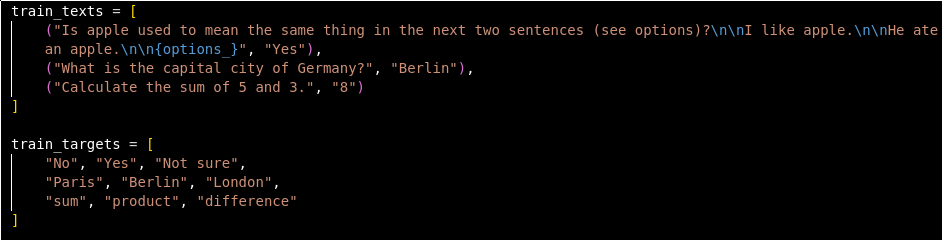
\includegraphics[scale=0.3]{png/p2.png}
		\item 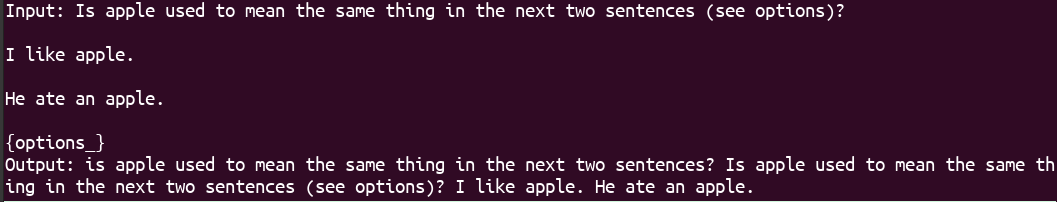
\includegraphics[scale=0.25]{png/p3.png}
		\item 只是重复了两遍.
	\end{itemize}

	
\end{itemize}
\end{frame}

\begin{frame}
	\frametitle{代码}
\begin{itemize}
	\item 时间序列的指令微调代码(t5\_finetuning.py)
	\eee{
		\item 程序有一些bug没跑通.
		\item 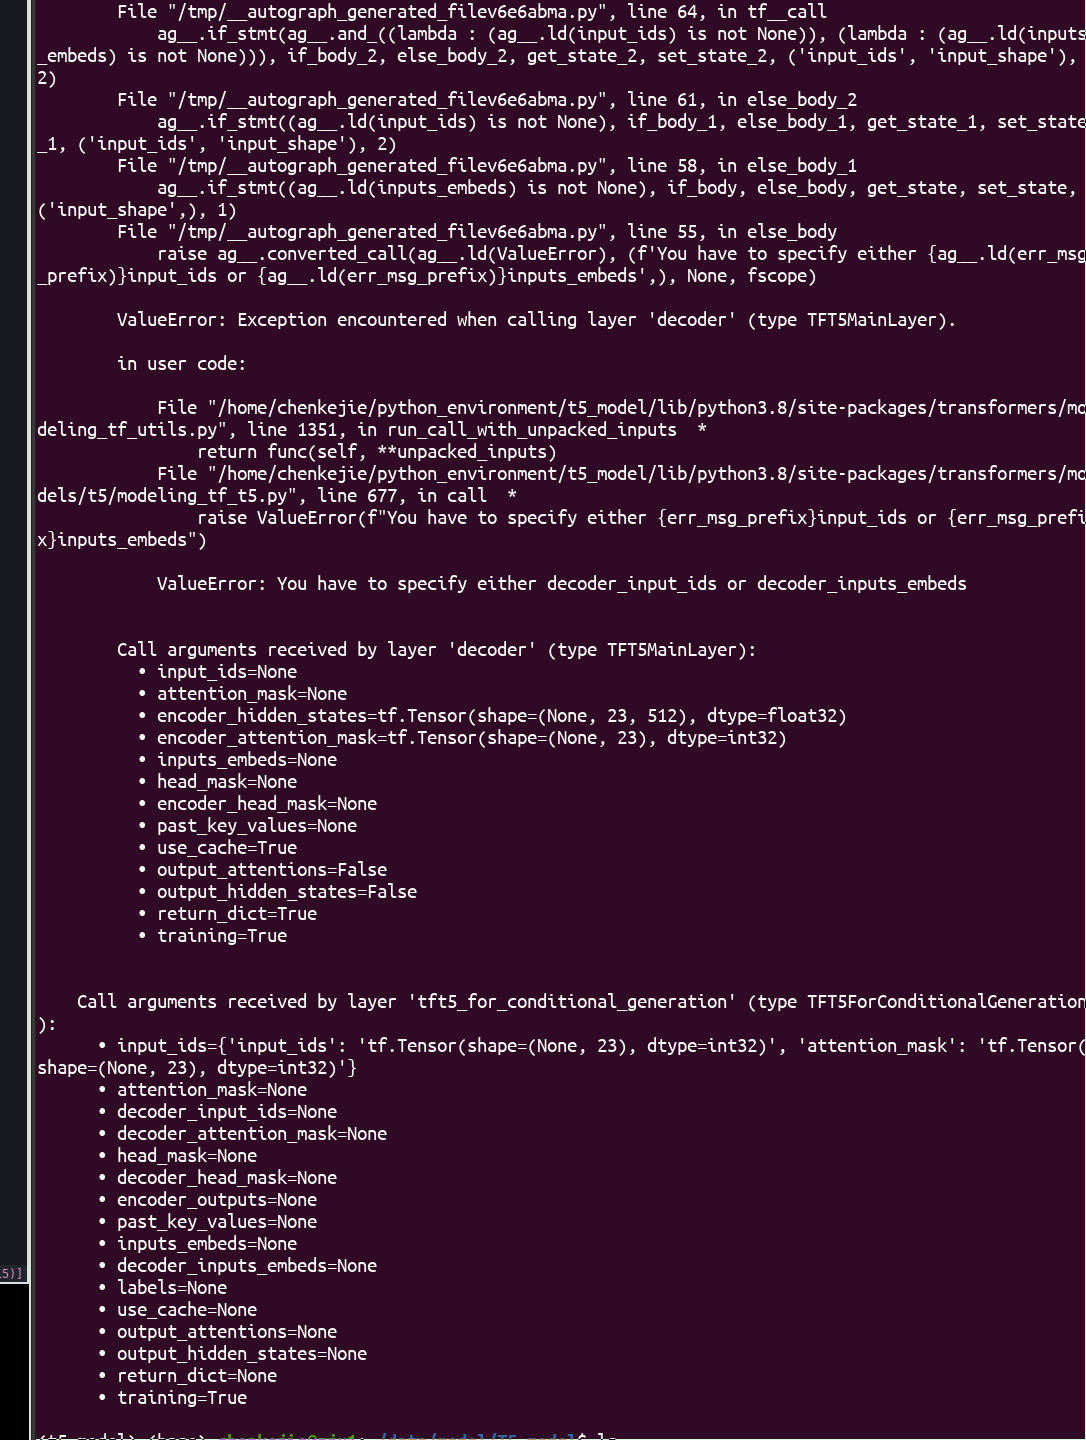
\includegraphics[scale=0.15]{png/p1.png}
				% \item TFT5ForConditionalGeneration模型是基于T5模型的条件生成模型,用于生成文本。在使用该模型时,需要提供decoder_input_ids或decoder_inputs_embeds参数来指定生成文本时的输入。
		% 根据报错信息,可以看到TFT5ForConditionalGeneration模型的调用参数中没有提供decoder_input_ids或decoder_inputs_embeds参数的值,导致报错。需要检查代码中关于生成文本输入的部分,确保提供了合适的参数。
		}
\end{itemize}
\end{frame}



\begin{frame}
	\frametitle{代码}
\begin{itemize}
	\item 时间序列的指令微调代码(t5\_finetuning.py)
	\eee{
		\item 在使用CUDA加速计算时,显存(GPU内存)不足以分配所需的张量。
		\item 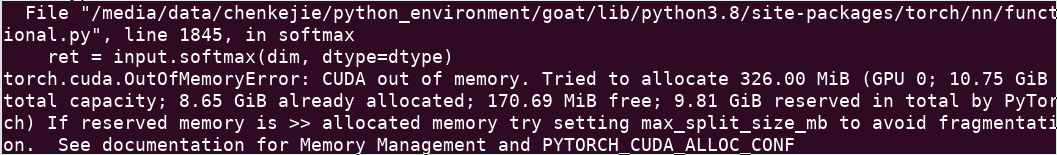
\includegraphics[scale=0.28]{png/bug.png}
		% \item TFT5ForConditionalGeneration模型是基于T5模型的条件生成模型,用于生成文本。在使用该模型时,需要提供decoder_input_ids或decoder_inputs_embeds参数来指定生成文本时的输入。
		% 根据报错信息,可以看到TFT5ForConditionalGeneration模型的调用参数中没有提供decoder_input_ids或decoder_inputs_embeds参数的值,导致报错。需要检查代码中关于生成文本输入的部分,确保提供了合适的参数。
		}
\end{itemize}
\end{frame}

\begin{frame}
	\frametitle{尝试运行如下几个程序:}
	\eee{
		\item Awesome-instruction-tuning:一个精心策划的开源指令调整数据集、模型、论文、资料库的列表。\\
		网址:\url{https://github.com/zhilizju/Awesome-instruction-tuning}
		\item stanford\_alpaca:该项目旨在建立和分享一个遵循指令的LLaMA模型。\\
		网址:\url{https://github.com/tatsu-lab/stanford_alpaca}
		\item Chinese-Vicuna:该项目旨在建立和分享遵循指令的中文LLaMA模型调整方法\\
		网址:\url{https://github.com/Facico/Chinese-Vicuna}
		\item FLAN:这个资源库包含了生成指令调谐数据集的代码。\\
		网址:\url{https://github.com/google-research/FLAN}
	}
\end{frame}


% 记得注释掉
% \begin{frame}
% 	\frametitle{llama模型}
% 	\eee{
% 		\item LLaMA (Touvron et al., 2023) 是一个集合
% 		训练有素的开源预训练语言模型使用公开数据集的数万亿个代币,并在许多方面实现了最先进的性能基准。
% 		先前的研究表明标记化对于 LLM 的算术能力很重要。 今天许多常用的子词标记化技术是不适合表示数字。 然而,美洲驼将每个数字拆分成一个单独的标记,从而确保数字的一致标记化,如附录 B 所示。
		
% 		语言模型的选择很重要我们的工作。 我们相信非凡的算术这项工作中展示的能力主要归功于 LLaMA 对数字。 我们通过实验验证其他LLM,例如 Bloom、OPT、GPT-NeoX 和Pythia,在相同的算术数据集上进行微调,无法匹配 LLaMA 的算术能力.
% 	}
% \end{frame}

% \begin{frame}
% 	\frametitle{test}
% 	\eee{
% 		\item LLaMA (Touvron et al., 2023) 是一个集合
% 		训练有素的开源预训练语言模型使用公开数据集的数万亿个代币,并在许多方面实现了最先进的性能基准。
% 		先前的研究表明标记化对于 LLM 的算术能力很重要。 今天许多常用的子词标记化技术是不适合表示数字。 然而,美洲驼将每个数字拆分成一个单独的标记,从而确保数字的一致标记化,如附录 B 所示。
		
% 		语言模型的选择很重要我们的工作。 我们相信非凡的算术这项工作中展示的能力主要归功于 LLaMA 对数字。 我们通过实验验证其他LLM,例如 Bloom、OPT、GPT-NeoX 和Pythia,在相同的算术数据集上进行微调,无法匹配 LLaMA 的算术能力.
% 	}
% \end{frame}



% 结束语
\section{}
\begin{frame}
	\frametitle{}
	\begin{center}
		\Huge{谢谢老师和同学的聆听!}
	\end{center}
\end{frame}


\end{CJK*}
\end{document}